% Converted from README.md
\subsection{Primer upotrebe KLEE alata}\label{primer-upotrebe-klee-alata}

Naredni primer (\texttt{01\_intro}) će nas sprovesti kroz osnovne korake pripreme izvornog koda za korišćenje alata. Razmotrimo kratak program u kome se testira funkcija koja proverava da li je učitan ceo broj paran:

\codefile{even.c}{c}

Možemo primetiti da je poslednja naredba u definiciji funkcije \texttt{even} nedostižna, odnosno da će se uvek izvršiti prvi ili drugi \texttt{return} u funkciji.

Priprema programa za simboličko izvršavanje:

\begin{enumerate}
\def\labelenumi{\arabic{enumi}.}
\tightlist
\item
  uključiti zaglavlje \texttt{klee/klee.h}
\item
  umesto učitavanja vrednosti promenljive koja nas zanima, označiti je simboličkom pomoću funkcije \texttt{klee\_make\_symbolic}
\item
  umesto korišćenja eksterne funkcije za ispis koju KLEE ne može da proveri, povratnu vrednost funkcije \texttt{even} ćemo vratiti preko povratne vrednosti funkcije \texttt{main}
\end{enumerate}

Argumenti funkcije \texttt{klee\_make\_symbolic}, redom:

\begin{enumerate}
\def\labelenumi{\arabic{enumi}.}
\tightlist
\item
  adresa promenljive
\item
  veličina promenljive
\item
  naziv promenljive (proizvoljna niska karaktera)
\end{enumerate}

Opciono: primetili smo da je poslednja linija funkcije \texttt{even} nedostižna, ali to možemo i potvrditi pozivom funkcije \texttt{klee\_assert(0)}, što će signalizitati grešku alatu ukoliko bude postojala putanja kojom se dolazi do poziva ove funkcije. U slučaju da takva putanja ne postoji, neće biti signalizirana greška i potvrdiće se pretpostavka da ne postoji ulaz za koji je ta naredba dostižna.

\textbf{Napomena:} Korišćenje funkcije \texttt{klee\_assert} zahteva uključivanje zaglavlja \texttt{assert.h}.

\begin{minted}{c}
#include <assert.h>
#include <klee/klee.h>

int even(int x) {
    if (x % 2 == 0)
        return 1;
    if (x % 2)
        return 0;
    klee_assert(0);
    return 1;
}

int main(int argc, char* argv[]) {
    int x;
    klee_make_symbolic(&x, sizeof(x), "x");
    return even(x);
}
\end{minted}

Pomoću Clang kompilatora generišemo LLVM bitkod koji će biti ulaz za KLEE (Clang će kreirati datoteku sa nazivom \texttt{even.bc}):

\begin{minted}{bash}
$ clang -emit-llvm -c -g even.c
$ klee even.bc
\end{minted}

\begin{minted}{text}
KLEE: output directory is "..."
Using STP solver backend

KLEE: done: total instructions = 42
KLEE: done: completed paths = 2
KLEE: done: generated tests = 2
\end{minted}

Na osnovu dobijenog izlaza, postoje dve putanje u našem programu, kao što smo i očekivali, u zavisnosti od toga da li je argument paran ili neparan po vrednosti. KLEE je generisao direktorijum pod nazivom \texttt{klee-out-0} sa test primerom za svaku eksploatisanu putanju. Pri sledećem pokretanju generisao bi se direktorijum \texttt{klee-out-1}, tj. u opštem slučaju direktorijum pod nazivom \texttt{klee-out-N} za prvo slobodno \texttt{N}. Takođe, napravljen je i simbolički link \texttt{klee-last} koji uvek ukazuje na poslednji \texttt{klee-out} direktorijum. Ukoliko izlistamo direktorijum \texttt{klee-out-0}, između ostalog, primetićemo datoteke sa ekstenzijom \texttt{.ktest}. To su binarne datoteke koje sadrže test primere za svaku putanju zasebno i koje se mogu pročitati korišćenjem alata \texttt{ktest-tool}:

\begin{minted}{bash}
$ ktest-tool --write-ints test000001.ktest
\end{minted}

\begin{minted}{text}
ktest file : 'test000001.ktest'
args       : ['even.bc']
num objects: 2
object    0: name: 'model_version'
object    0: size: 4
object    0: data: 1
object    1: name: 'x'
object    1: size: 4
object    1: data: 0
\end{minted}

\begin{minted}{bash}
$ ktest-tool --write-ints test000002.ktest
\end{minted}

\begin{minted}{text}
ktest file : 'test000002.ktest'
args       : ['even.bc']
num objects: 2
object    0: name: 'model_version'
object    0: size: 4
object    0: data: 1
object    1: name: 'x'
object    1: size: 4
object    1: data: 1
\end{minted}

Primećujemo da je KLEE generisao ulaz \texttt{0} i \texttt{1} za pokrivanje dve otkrivene putanje, tj. jednu parnu i jednu neparnu ulaznu vrednost.

Da bismo proverili da li naš program daje očekivane izlaze za generisane test primere, možemo testirati polazni program korišćenjem vrednosti \texttt{data} iz pročitanih testova ili koristiti simbolički program zahvaljujući posebnoj biblioteci \texttt{libkleeRuntest} i koja pozive funkcije \texttt{klee\_make\_symbolic} zamenjuje pozivom funkcije koja promenljivoj dodeljuje vrednost zapisanu u odgovarajućoj test datoteci.

Testiranje pomoću \texttt{libkleeRuntest} biblioteke:

\begin{minted}{bash}
$ export LD_LIBRARY_PATH=/putanja/do/klee/Release+Asserts/lib
$ gcc \
    -I /putanja/do/klee/include/ \
    -L /putanja/do/klee/Release+Asserts/lib even.c \
    -lkleeRuntest
$ KTEST_FILE=klee-last/test000001.ktest ./a.out
$ echo $?
1
$ KTEST_FILE=klee-last/test000002.ktest ./a.out
$ echo $?
0
\end{minted}

Očekivano, nismo dobili poruku od \texttt{klee\_assert} što potvrđuje pretpostavku da je označen deo koda nedostižan za bilo koji ulaz.

Statističke informacije u vezi sa izvršavanjem KLEE alata nad nekim bitkodom, kao što su broj izvršenih instrukcija, pokrivenost instrukcija bitkoda, pokrivenost grana bitkoda i slično, možemo dobiti pomoću Python skripta \texttt{klee-stats}. Informacije se prikazuju u tabelarnoj formi. Ovaj alat se poziva nad direktorijumom koji je generisao KLEE. Da bismo bili sigurni da je to najnovija verzija direktorijuma, najjednostavnije je alat pozvati sa argumentom \texttt{klee-last}.

\begin{minted}{bash}
$ klee-stats klee-last
\end{minted}

\begin{minted}{text}
------------------------------------------------------------------------
|  Path   |  Instrs|  Time(s)|  ICov(%)|  BCov(%)|  ICount|  TSolver(%)|
------------------------------------------------------------------------
|klee-last|      42|     0.06|    12.16|     5.71|     296|       90.36|
------------------------------------------------------------------------
\end{minted}

Legendu za tabelu možemo dobiti pomoću opcije \texttt{-{}-help}.

\begin{minted}{text}
LEGEND
--------  ---------------------------------------------
Instrs    number of executed instructions
Time      total wall time (s)
ICov      instruction coverage in the LLVM bitcode (%)
BCov      branch coverage in the LLVM bitcode (%)
ICount    total static instructions in the LLVM bitcode
TSolver   time spent in the constraint solver
\end{minted}

Vizuelni prikaz statistike o simboličkom izvršavanju možemo dobiti korišćenjem alata \emph{KCachegrind}:

\begin{minted}{bash}
$ kcachegrind klee-last/run.istats
\end{minted}

Izborom \texttt{CoveredInstructions} ili \texttt{UncoveredInstructions} i izborom kartice \texttt{Source\ Code} možemo tačno videti koje linije jesu, odnosno nisu pokrivene test primerima.

\pandocbounded{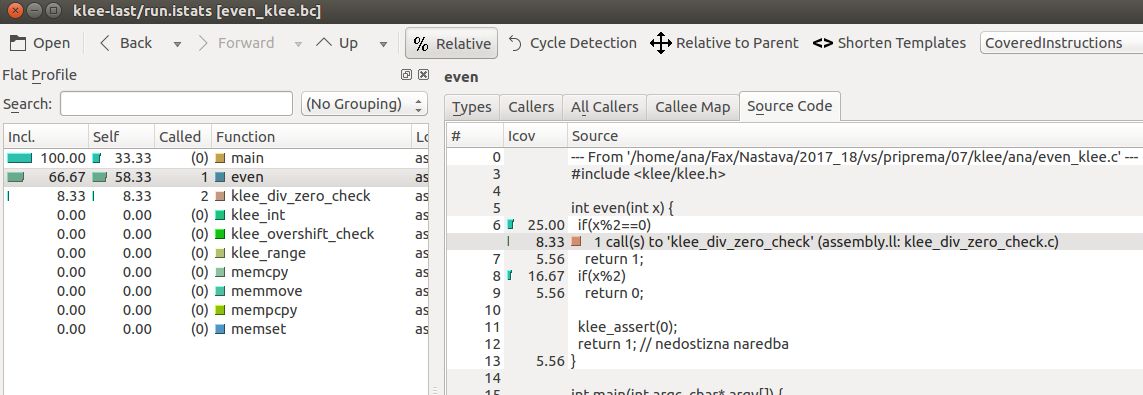
\includegraphics[keepaspectratio]{images/kcache_coverage.png}}

Primetimo da su brojevi koje sada vidimo daleko veći od brojeva koje je prikazao \texttt{klee-stats}. Razlog je to što gcov razmatra samo linije u jednoj datoteci, a ne u celoj aplikaciji, dok sa KCachegrind-om možemo čitati izlaz gcov-a o pokrivenosti koda i ispratiti koje su linije pokrivene, a koje ne.
